%%%%%%%%%%%%%%%%%%%%%%%%%%%%%%%%%%%%%%%%%%%%%%%%%%%%%%%%%%%%%%%%%%%%%%%%%%%%
%% Trim Size : 11in x 8.5in
%% Text Area : 9.6in (include Runningheads) x 7in
%% ws-jai.tex, 26 April 2012
%% Tex file to use with ws-jai.cls written in Latex2E.
%% The content, structure, format and layout of this style file is the
%% property of World Scientific Publishing Co. Pte. Ltd.
%%%%%%%%%%%%%%%%%%%%%%%%%%%%%%%%%%%%%%%%%%%%%%%%%%%%%%%%%%%%%%%%%%%%%%%%%%%%
%%

%\documentclass[draft]{ws-jai}
\documentclass{ws-jai}
\usepackage[flushleft]{threeparttable}
\begin{document}

\catchline{}{}{}{}{} % Publisher's Area please ignore

\markboth{P.Prasad}{The AARTFAAC Radio Sky Monitor: System Design and Implementation}

\title{The AARTFAAC Radio Sky Monitor: System Design and Implementation}

\author{Peeyush Prasad$^\dagger$, Folkert Huizinga$^\dagger$, Eric Kooistra$^\ddagger$, Daniel van der Schuur $^\ddagger$, Andre Gunst $^\ddagger$ and R.A.M.J. Wijers$^\dagger$}

\address{
$^\dagger$Anton Pannekoek Institute, Universitiet van Amsterdam, Amsterdam, The Netherlands, fauthor@university.com\\
$^\ddagger$ASTRON, Oude Hoogeveensedijk, 7991PD, The Netherlands\\
$^\S$Group, Company, Address, City, State ZIP/Zone, Country, fauthor@company.com
}

\maketitle

\corres{$^\dagger$Peeyush Prasad.}

\begin{history}
\received{(to be inserted by publisher)};
\revised{(to be inserted by publisher)};
\accepted{(to be inserted by publisher)};
\end{history}

\begin{abstract}
The Amsterdam-ASTRON  Radio Transients  Facility And Analysis  Center (AARTFAAC)
array  is  a sensitive,  all-sky  radio  transient  detector  based on  the  Low
Frequency Array (LOFAR).  It generates images  of the low frequency radio sky in
near real-time  with spatial resolution of  10s of arcmin, MHz  bandwidths and a
time cadence of a few seconds. The image timeseries are then monitored for short
and bright radio  transients. On detection of a transient,  low latency triggers
will be  generated for LOFAR,  which can  carry out follow-up  observations.  In
this  paper, we  describe our  heterogenous, hierarchical  design to  manage the
~1.2Tbps raw  data rate, and the  ~17TFLOPs of computing needed.  We discuss the
implementation of the instrumentation, and its capabilities
\end{abstract}

\keywords{Radio Interferometry, Imaging, Radio Transients, Correlators}

\section{\label{sec:Introduction}Introduction}

\begin{itemize}
\item What are celestial transients \\
\noindent Transient astronomy deals  with the detection and  characterization of celestial
transients, sources in  the sky whose detectable properties can  change on short
timescales.   These  explosive   events  provide  insight  into   a  variety  of
astrophysics,  ranging from  emission mechanisms  of jets  to properties  of the
intervening  medium [ref].  There is  a rich  history of  the detection  of such
objects  across  wavelength  ranges,  with  each  wavelength  regime  probing  a
different parameter space [ref].

\item Current  state of  radio instrumentation\\
Studies of short  duration radio emission from such objects  has been restricted
to either very  short timescales (milliseconds to seconds, e.g.  Pulsars), or to
comparitively longer timescales (months to  years) primarily due to instrumental
or observational time constraints, the latter  due to the narrow fields of view.
Radio instrumentation is available in broadly two classes; single dish or phased
array  beam  formed   timeseries  characterized  by  high   time  and  frequency
resolution,  fields of  view  of  a few  degrees  but  poor spatial  resolution.
Aperture  synthesis imaging  observations  address the  latter  to provide  high
spatial resolution,  but have  poor time  resolution, typically  needing several
hours of  observation time  to build up  adequate coverage in  the UV  plane via
earth  rotation aperture  synthesis.   The above  classes  roughly translate  to
coherent  (short  timescales)  and  incoherent (longer  timescales)  sources  of
emission.

\item Current state of the science \\
The serendipitous discovery of a new  class of radio transient termed Fast Radio
Bursts  (FRBs) has  galvanized  interest in  the field.  The  detected FRBs  are
characterized by high associated dispersion  measures, high brightness and short
timescales.  They are  non-repeating for  the  most part.  Their unknown  origin
requires  not  only their  discovery,  but  also  rapid  followup over  a  large
wavelength regime to establish emission phenomena and associated parameters.

The last requirement has led to the development of large field of view radio sky
monitors, with an  aim of continuously surveying large parts  of the visible sky
with shallow sensitivity and at high  time resolution. A trigger is generated on
the reliable  detection of  a transient  in close  to real-time,  allowing other
telescopes to carry out follow-up observations.

\item Suitability of low frequency observations \\
<TODO: Paragraph about  transient sources, some stuff about  spectral indices of
coherent emission and  expected class of sources, at what  brightness levels can
we expect to see things (take from Lazio LWA paper).>

<TODO: Paragraph  summarizing the  current state of  knowledge of  low frequency
transients: Stewart NCP transient, other  searches at low freq. Conclusion: Need
for more monitoring.>

\item What is the AARTFAAC \\
The AARTFAAC  radio transient  monitor is  an All-sky  radio telescope  based on
LOFAR. Its goal is to continuously scan  the skies for bright transients, and on
reliably detecting one, to generate a trigger to other telescopes for sensitive,
broad  band monitoring.   It is  a leading  effort among  a group  of new  radio
telescopes  aiming for  detection  of  bursts of  radio  emission by  continuous
monitoring of the low radio frequency sky.  Such telescopes are characterized by
having  moderate   resolution  and  sensitivity  as   compared  to  contemporary
telescopes, but  with extremely wide  fields of  view (typically all  sky), high
availabilities and autonomous calibration and imaging in near real-time.

The  latter  requirements are  unconventional  by  contemporary Radio  Astronomy
standards, and make their implementations challenging. The antenna elements used
to achieve  the wide fields  of view are  typically dipoles, however,  their low
individual  sensitivities  requires  an  order of  magnitude  larger  number  of
elements in the array.  Bringing the resulting large number of data streams to a
central  location,  as well  as  their  correlation  for carrying  out  aperture
synthesis  imaging  in  real-time  thus  poses a  significant  I/O  and  compute
challenge. Further,  the wide fields of  view at the sensitivities  of operation
also result in  direction dependent effects on the incoming  signals, mostly due
to  the ionosphere.  These  pose  a challenge  to  calibration, especially  when
carried out in an autonomous manner.

Apart  from  its  primary  goal  of  trigger  generation  on  the  detection  of
transients, the telescope products find use in a variety of science cases. These
include  wide  field  ionospheric  monitoring via  apparent  flux  and  position
variations of  calibrator sources, Solar  monitoring, RFI surveying,  LOFAR beam
model validation etc.

\item AARTFAAC as a data transport, reorganization and computing problem.\\
The  wide field  of  views necessary  for  an instrument  like  AARTFAAC can  be
achieved by sampling the sky with wide field dipoles. This, however comes at the
cost  of lowered  sensitivity per  receiving element.   An instantaneously  well
sampled  UV  plane  is  needed  to  generate a  PSF  with  low  sidelobes.  Both
requirements can be  met by spatially spreading a large  number of dipoles.  The
highest sensitivities  can also be achieved  by the coherent correlation  of the
incoming  signal,  requiring  access  to  the nyquist  sampled  signal  at  full
resolution. Such an arrangement then  requires the aggregation of high bandwidth
data from the receiver elements, necessitating a high speed data network.

The incoming  sampled voltages  pass through  various signal  processing blocks,
resulting  in the  generation of  light curves  for sources  in the  image.  The
estimation of spatial coherences requires the reordering of data to make optimum
usage of  compute resources. Thus, the  functioning of the telescope  depends on
the optimization of the data  transport, data reorganization and computing using
available resources.   An advantage of  having an operating model  consisting of
signal   processing  blocks   operating   on  high   resolution   data  is   the
configurability of the telescope into different  observing modes, as well as the
tapping  off of  data from  an upstream  location.  The  latter ability  makes a
piggy-back  instrument like  the  AARTFAAC possible.  An  important resource  to
optimize is the development time for  each data routing or processing block, and
this has been taken into consideration in the AARTFAAC.

\item Paper description \\
In  this paper,  we describe  the  AARTFAAC telescope  system architecture,  its
instrumentation,  and  the commissioning  of  its  various subsystems.   Section
\ref{sec:aartfaac_array} describes the array and the receiving antenna elements,
its  relationship  with LOFAR,  and  introduces  the  full architecture  of  the
instrument.    Section   \ref{sec:station_hardware}   describes   the   hardware
implementation in  the field which  allows creating a  data path in  parallel to
LOFAR. This  makes AARTFAAC processing independent  of LOFAR to a  large extent.
In Section \ref{sec:gpucorr}, we describe the implementation of a real-time, GPU
based  correlator  for  AARTFAAC,  while  Section  \ref{sec:calim}  details  the
real-time,   autonomous  calibration   and   imaging  implementation.    Section
\ref{sec:acontrol} describes our  control system for the  full instrument, which
also interfaces with LOFAR.  In Section \ref{sec:results} we present performance
metrics of the instrument as a whole.
\end{itemize}

\section {\label{sec:aartfaac_array}The AARTFAAC array}
We  begin by  summarizing the  subsystems of  the LOFAR  telescope relevant  for
AARTFAAC processing in  Section \ref{subsec:lofar}, and then  elaborating on the
scheme for creating a coupled data path for independent processing by AARTFAAC.

\subsection {\label{subsec:lofar} LOFAR telescope architecture}
The LOFAR telescope \ref{} is a new generation radio interferometer covering the
frequency  range from  10-90  MHz using  inverted V-dipoles  known  as Low  Band
Antenna (LBA),  and from 110-240  MHz using Bowtie  dipoles, also known  as High
Band  Antenna (HBA).   The  antenna are  linearly polarized,  being  made up  of
orthogonally  placed  dipoles in  the  E  and H  plane.  The  LBA dipole  has  a
sensitivity pattern  with a 6dB  field of view of  about $120^o$, while  the HBA
dipoles first undergo  an analog phasing within  a 4x4 tile, which  results in a
field  of view  of  about TODO.  Due  to this  restriction,  the AARTFAAC  array
utilizes only the LBA part of the telescope.

The  telescope itself  consists of  a  large collection  of antennas,  spatially
organized into several 'stations', each spread  over ~60m. The stations are laid
out in a  dense core: 24 (TODO:  Check) stations within a 2km  radius, while the
long baselines  of stations of  upto a 1000km are  also present. At  the station
level, the  received and conditioned analog  signals from a dipole  are baseband
sampled with a 200MHz clock and  10-bit quantized.(TODO: Check). The signal from
each  polarization  is then  split  into  spectral  subbands  of ~200kHz  via  a
polyphase  filterbank  implementation.   In  the  regular  LOFAR  station  level
processing, the  dipole subbands are  then digitally phased in  hardware towards
the direction of  an astronomical source to  form a station beam,  which is then
transmitted over optical fiber for further interferometric processing with other
stations.

The LOFAR correlator architecture needs real-time processing to reduce the large
volume of  data being  produced. Its  implementation is also  based on  a hybrid
architecture using  GPGPUs and  CPUs. [TODO:  Should this  be mentioned  at all?
  Might weaken the case, with our implementation being very similar to the LOFAR
  case.]

A  schematic  representation   of  the  LOFAR  level  processing   is  shown  in
Figure. TODO

\subsection {\label{subsec:aartfaac}  The AARTFAAC system}
The AARTFAAC  array consists of  12-stations from within  the core of  the LOFAR
telescope, with interdipole distances ranging  from (TODO) within a station, and
a maximum of TODO across stations.  Due  to the requirement of dipole level data
in order to achieve all-sky imaging, the AARTFAAC creates a coupled data path to
an independent processing  architecture, prior to the phasing up  of the dipoles
in the  LOFAR processing  flow. This allows  simultaneous observing  with LOFAR,
leading to high  availability of the AARTFAAC system. A  subset of the available
subbands are  correlated in a dedicated  GPU based correlator in  real-time. The
estimated visibilities  are sent over  TCP/IP to dedicated servers  for carrying
out the autonomous and real-time  calibration and imaging.  The generated images
are further sent to a software  pipeline for the actual detection of transients,
based on  comparison of  the image timeseries.   A (planned)  trigger generation
subsystem  will publish  reliable triggers  in the  form of  VOEvents [refTODO],
which  can be  claimed  by  other telescopes  to  observe  candidates with  high
sensitivity and resolution.

\subsubsection {\label{subsubsec:arrayconf} Array configuration}

\begin{figure*}[htbp]
\centering
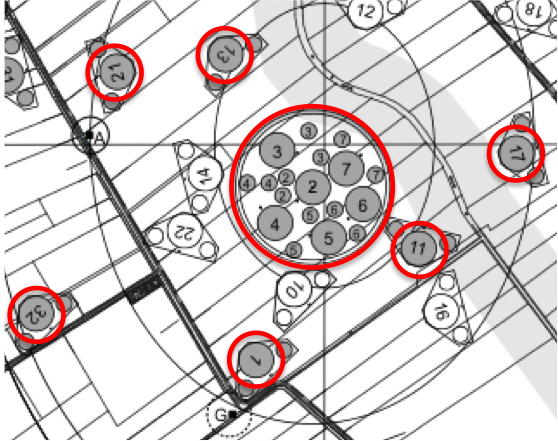
\includegraphics[width=0.25\textwidth]{Figs/afaac12_arrayconfig.png}
\caption{The spatial distribution of AARTFAAC-12 stations within the core of LOFAR stations.}
\label{fig:afaac12_arrayconfig}
\end{figure*}

The choice of stations is dictated primarily by imaging quality and sensitivity,
but  also due  to constraints  on the  latency of  calibration and  imaging. The
central  six stations  of  the LOFAR  telescope (called  the  superterp) form  a
densely sampled UV plane,and are ideal for wide field imaging due to their being
co-planar to  high accuracy (centimeter  level). The outer six  stations provide
higher  sensitivity  and resolution.  The  salient  features of  the  LBA\_OUTER
station configuration  for the chosen stations  are shown in table  TODO. Figure
\ref{fig:afaac12_arrayconfig}  shows the  LOFAR stations  that are  part of  the
AARTFAAC system.

TODO: Add 12-station beam characteristics, expected confusion noise contribution.

\begin{figure*}[htbp]
\centering
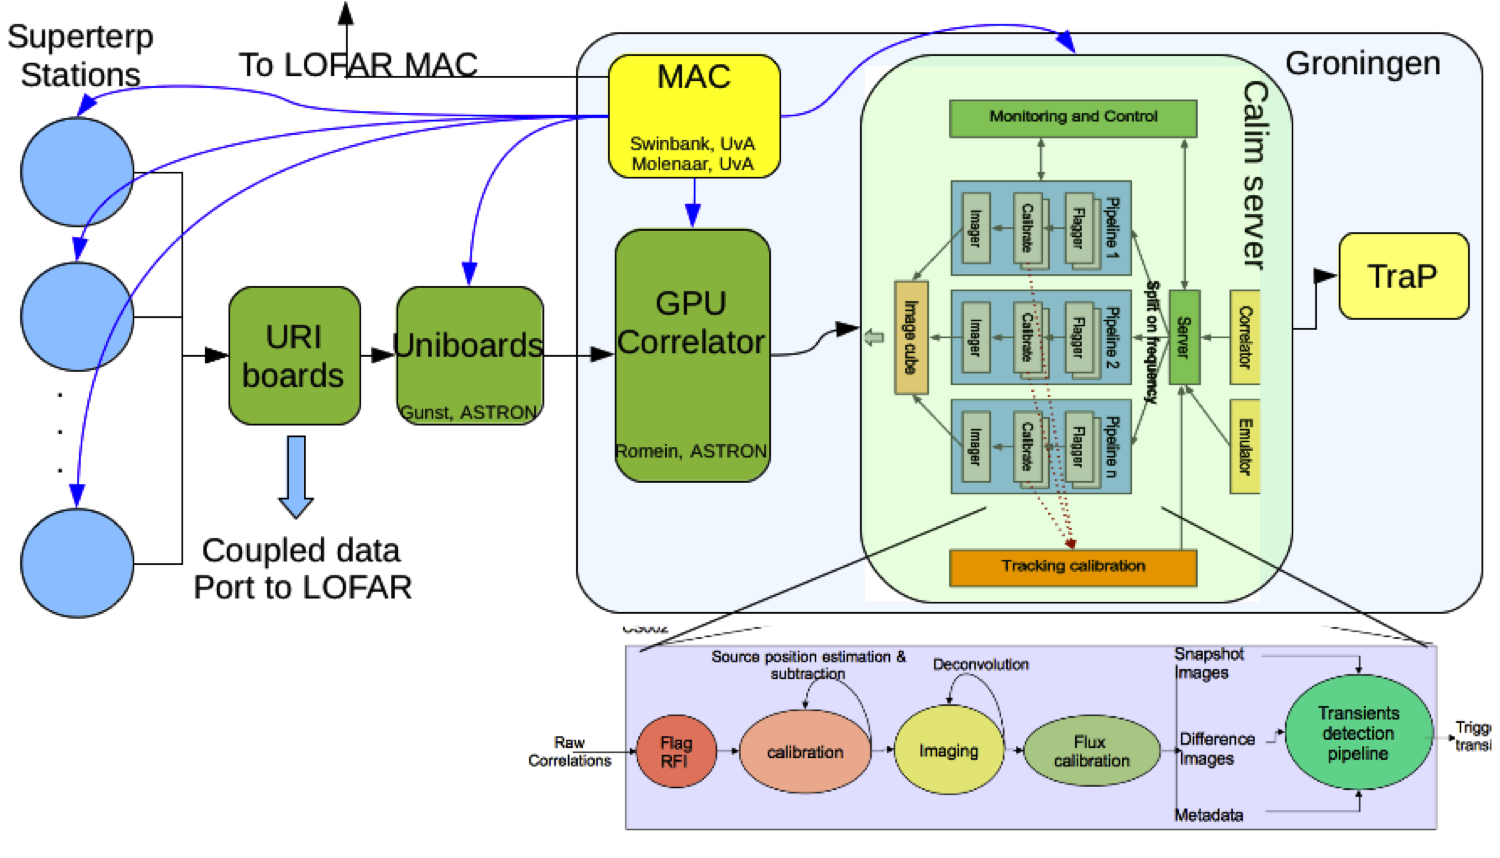
\includegraphics[width=1\textwidth]{Figs/overall_afaac_Arch_blks.png}
\caption {Overall  architecture of the  AARTFAAC all-sky monitor  depicting each
  processing subblock.}
\label{fig:afaac_arch}
\end{figure*}

The station  consititute the first component  of the radio sky  monitor, and are
the only components shared with LOFAR.  The AARTFAAC monitor consists of further
subsystems which are independent of  LOFAR processing.  Its overall architecture
is shown schematically in Figure  \ref{fig:afaac_arch}, and illustrates the main
processing subblocks of the instrument.   To summarize, a user selectable subset
of subbands  from every dipole  is transferred as  UDP packets over  a dedicated
10Gbit fiber connection  to the central processing systems.   These are received
by  a streaming  software correlator  implementation which  aligns the  data and
estimates  the spatial  covariance matrix  between every  pair of  dipoles.  The
generated visibilities  are streamed  over TCP/IP to  a calibration  and imaging
pipeline component  which carries out  autonomous imaging.  The images  are then
analyzed by a software tool (The  Transients Pipeline, TraP), which extracts the
light curves  of sources  within the  image, and  analyses them  for variability
using a number of parameters. The TraP is described in more detail in \ref{}.

The  specifications of  the  AARTFAAC  monitor are  listed  in  Table TODO.   We
describe the  various subsystems making up  the AARTFAAC All-sky monitor  in the
following sections.

\section {\label{sec:station_hardware} Remote Station Level Processing:} 
Remote  Station processing  refers  to instrumentation  installed  in the  field
coupled to the receiving antennas post balun. This consists of Digital Converter
Unit (DCU)  boards and the  Remote Station  Processing (RSP) boards.  The former
caters to analog  signal conditioning of the received voltage,  followed by base
band digitization  at 200MHz, with TODO bit resolution.\\

The RSP boards handle the reception of  sampled voltages from the DCU boards and
their first stage  processing. In the following, we describe  the parts relevant
to  the functioning  of  the  AARTFAAC telescope.   The  RSP  board consists  of
TODO NUM TODO TYPE  FPGAs, with  TODO input bandwidth  over TODO  connector, and
TODO output bandwidth  over TODO connector.  [TODO Add  reference] describes the
implementation of this board  in more detail. A single RSP  board can handle the
processing of sampled data from 4 dual polarized dipoles.  Since a LOFAR station
is made up of 48 dual polarized dipole antennas, 12 such boards are required per
station.\\

\textbf {Signal processing:} The RSP board carries out the first stage polyphase
filter bank  implementation common  to the LOFAR  and AARTFAAC  telescopes. This
filter bank  analyzes the voltage timeseries  sampled at 200 MHz  available from
the samplers, into a complex voltage  spectrum of 512 subbands. Thus, the entire
analog band of the LBA between 10-90MHz is available for further processing. The
output, for a set of 1024 real  voltage samples, consists of fixed point complex
values per subband.  These values fundamentally have a 16-bit  resolution on the
real and imaginary components. [Add some more on dynamic range expected etc.]\\

Station level  beamforming in  a particular  direction requires  calculating the
weighted sum of  all dipoles of the same polarization,  with the applied weights
being dependent on  the direction of beamforming.  Each  RSP board fundamentally
generates the  beamformed product for  its 4  client dipoles for  every subband.
These are termed  as 'beamlets'.  The necessary exchange of  beamlets with other
RSP boards to  create the station beam is achieved  via the interconnect between
the various RSP boards.\\

Each data  product from the RSP  signal processing is encapsulated  in a packet,
and marked with a datatype magic number. This allows differentiation between the
generated data products.

\textbf  {Interconnect:}  A  ring  network  consisting  of  four  10-GigE  links
interconnects    the    RSP   boards    to    each    other,   as    shown    in
Fig. \ref{fig:afaac_station_hw}.  It is implemented  by daisy chaining  the GigE
links of  the RSP  boards to  each other. It  carries beamlet  data, and  has an
AARTFAAC specific mode  (enabled only on AARTFAAC boards? TODO  check) where the
raw subbands  for every dipole polarization  are also transferred onto  the ring
network. Of the total TODO bandwidth of the ring network, about TODO is occupied
by  LOFAR specific  products. The  remaining  bandwidth carries  the per  dipole
subbands, which are used exclusively for AARTFAAC processing.\\

The fundamental limitation  to AARTFAAC processed bandwidth is  presented by the
interconnect, and  depends on the  bit-mode chosen.  The bandwidth  available to
AARTFAAC is limited to 36 subbands in 16-bit mode, 72 subbands in 8-bit mode, or
144 subbands in 4-bit mode. The bit modes are mutually exclusive, and can be set
via control  registers.  A random selection  of subbands from the  available 512
can be inserted into the available slots on the interconnect. This selection can
be made via manipulation of the control registers of the RSP board.  This allows
AARTFAAC to achieve high sensitivity by placing subbands contiguously, and later
integrating them, while at the same  time achieving spectral coverage by placing
subbands to sample a larger extent of the analog spectrum.

\textbf  {Available bit  modes:}  The system  offers the  ability  to trade  off
dynamic range in  the polyphase filter bank outputs with  the number of subbands
available  for further  processing.  This  is done  by  reducing  the number  of
allocated bits  to the  real and  imaginary components  of the  subband outputs,
leading to an increased number of subbands.  The bit mode of AARTFAAC can be set
completely independently of  LOFAR's choice of bit mode. The  choice between the
various bit modes  depends on the RFI environment of  the observation.[TODO: How
  is the  data converted  from 16-bit to  8-bit? Which 8-bits  are taken  as the
  output?  Implications?].  An  8-bit complex  representation of  the filterbank
outputs  is found  to be  adequate for  almost all  observing conditions  except
during severe RFI.

\textbf {Sampling  clock and Timing:}  A clock  distributer board [TODO  REF] is
used  to  distribute  a  10MHz  reference  to  every  one  of  the  12  AARTFAAC
stations. This  reference is  generated by a  GPS discplined  Rubidium frequency
standard. This ensures that an identical  (hence coherent) clock is used for the
sampling of data from the AARTFAAC stations.\\

Every station is equipped with a Local  Control Unit (LCU), which is an embedded
(TODO:Check?)  processor  running a Linux  operating system.  These  systems are
networked to the LOFAR control system, and  also act as NTP clients. Thus, their
absolute times are aligned to better than a few milliseconds. This absolute time
from the station LCU is communicated to  the RSP board [TODO: Check?] on station
reset, as the  reset value to a  64bit counter.  Once set,  the station hardware
updates  this counter  on a  derivate of  the available  200MHz reference,  thus
ensuring that  the absolute  time is  embedded in the  data with  few nanosecond
[TODO check] resolution. All further aligning and timing of the incoming data is
carried out based on this embedded timestamp.

\textbf {The Uniboard-RSP  Interface (URI) board:} This  AARTFAAC specific board
creates a coupled path  for the subband data by segregating  them from the LOFAR
specific data products flowing on the  station ring network. This is implemented
by interfacing  the interconnet  of 4 RSP  boards to a  single URI  board, which
interrogates  the incoming  packets, and  selects the  subband outputs  based on
packet type.  This block  further implements  the first  stage of  the necessary
swizzle  operation by  statically  routing a  subband from  all  dipoles of  the
station to a single output lane.[Add more detail here.]\\

All together, three URI boards are  adequate to transfer and swizzle 36 subbands
at 16-bits into the uniboard based router.

\textbf  {The  Uniboard based  data  router:}  This  data  routing unit  is  the
interface  between  the  station  level instrumentation,  and  the  next  signal
processing unit, the correlator. It fundamentally consists of 4 upstream (called
backnodes) and 4 downstream (called frontnode) FPGAs. Each of the backnode FPGAs
receives 8 consecutive subbands out of the  36 subbands in the URI board output,
making 32  subbands available to  the Uniboard. A  second level of  swizzling is
carried out at this stage via physical routing of subbands between the URI board
and the  Uniboard. The  resulting stream out  of a backnode  FPGA consists  of 8
subbands of all 48 dipoles of a  station. These data are transported to a single
Frontnode FPGA.   The latter encapsulates  the data into  a UDP packet  which is
transmitted  on  a  long  haul   10Gigabit  Ethernet  interface  to  the  remote
correlator.  A  single  Uniboard  operates  two  10Gbps  links  to  the  central
processing machines, located at the University of Groningen about 50Km away.


\textbf  {Subband data  format:}  (Is this level of detail needed?)
\textbf {Commissioning effort and Performance:}

\textbf {Data rates and bandwidth limitations: } The stations operate on a fixed
sampling  clock of  200 MHz,  leading to  an output  rate of  ~12 Mbps  per dual
polarised dipole  antenna per 16-bit  complex subband. The limited  ring network
bandwidth of a station  allows only 36 of the available  512 subbands of 16-bits
from all  dipole antennas  (total bandwidth  ~20Gbps) to be  carried to  the URI
board.  The  station Uniboard further  restricts the sampled bandwidth  to match
its output bandwidth into 2x10Gbps links.   Of the incoming 36 subbands, only 16
are  forwarded   for  correlation.   Each  10Gbps   link  carries   8  subbands,
corresponding to ~4.5Gbps of data.


\textbf  {Control interface:}  The  control of  the  remote station  electronics
consists of  two layers. At  the FPGA level,  command and status  registers have
been opened up.  These can be accessed  via the a separate  (TODO: Double check)
control Gigabit Ethernet  interface. Each station is also equipped  with a Local
Control  Unit  (LCU)  computer  which  provides  an  abstraction  layer  to  the
hardware. All control  and monitoring commands from a global  control system are
addressed  to the  LCU,  which provides  a  tool that  can  access the  hardware
registers  via a  driver, which  ultimately communicates  the commands  over the
Gigabit ethernet control link to the RSP boards of the station.

\begin{figure*}[htbp]
\centering
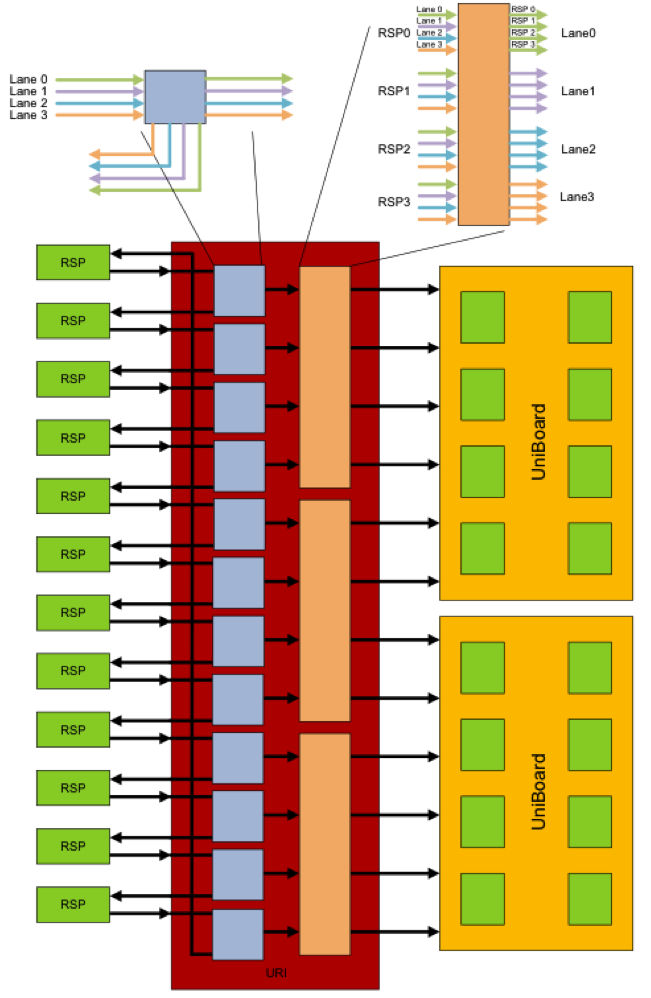
\includegraphics[width=0.75\textwidth]{Figs/station_hw_proc_afaac.png}
\caption{The station level hardware changes  allowing creation of a coupled data
  path for AARTFAAC data flow.}
\label{fig:afaac_station_hw}
\end{figure*}

Figure \ref{fig:afaac_station_hw} depicts the  station level ring network, whose
bandwidth is shared between the beamformed  subbands as well as the dipole level
subbands. The ring network bandwidth constrains the processed AARTFAAC bandwidth
to  a fundamental  maximum of  36 16-bit  subbands, or  about 7  MHz, while  the
Uniboard  interface further  restricts the  bandwidth to  8 subbands  per 10Gpbs
output link. The URI boards in combination  with the uniboards carry out a first
level of the incoming data transposition.

\section {\label{sec:gpucorr} The AARTFAAC real-time correlator}
\begin{figure*}[htbp]
\centering
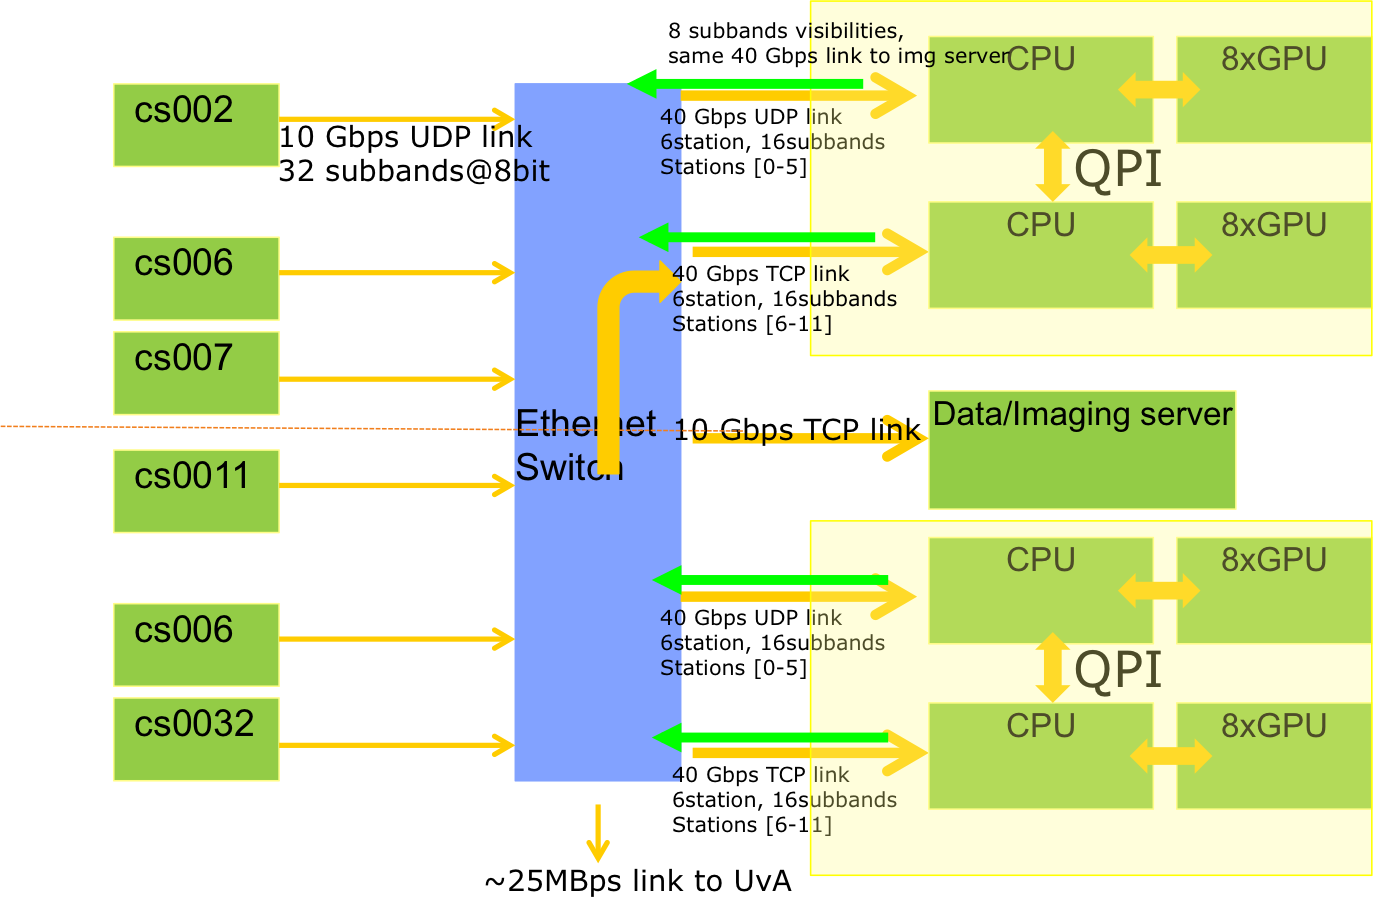
\includegraphics[width=1\textwidth]{Figs/correlator_arch.png}
\caption{The GPU  correlator implementation  using a pair  of Xeon  class server
  machines hosting AMD GPUs}
\label{fig:afaac_station_hw}
\end{figure*}

\begin {itemize}
\item What does the correlator do\\
The correlator  subsystem estimates the  spatial coherence between all  pairs of
the 1156  polarizations of the  drooped dipoles, per  subband.  This is  done by
computing  the  average  cross  correlation  between  antenna  polarization  per
subband. Its  input is formed of  the subbanded complex voltage  timeseries from
each  polarization  of every  antenna.   The  output  consists  of a  stream  of
visibilities with a chosen time and  frequency averaging.

\item The correlator  requirements for AARTFAAC \\ 
The AARTFAAC  correlator must estimate  the correlation from 1152  input streams
with as  little latency as possible.  It thus needs  to ingest a very  high data
rate.  Further,  it  should  be  able  to  produce  channelized  output  due  to
requirements of RFI  flagging, while being configurable in  its time integration
capabilities.  A major requirement of the implementation was that of development
time, which effectively eliminated a firmware based approach.

\item Motivating the GPGPU approach\\
Of the available approaches, an heterogenous GPGPU approach turned out to be the
best match between our requirements of  ease of development and performance. The
correlation operation  has a  low Arithmetic Intensity,  implying that  the data
brought to a device ALU is operated on only a few times. This, combined with the
relatively restricted I/O bandwidth between the host CPU and the device GPU, has
been used as  an argument against using GPGPU systems  for correlation. However,
with increasing number  of signal sources, the I/O  requirements scale linearly,
while the compute  requirements scale quadratically. Thus, a  large enough input
system can make the application compute bound. This is the case withthe AARTFAAC
system. Assuming the input subbands from the 1152 dipole elements would be split
into 64 channels, with a one second time integration, the total required compute
power required is ~17 TFLOP/sec. The latest GPUs come close to this requirement.

\item Functional blocks \\
The signal processing blocks necessary to achieve the correlator specs are shown
in Fig. TODO.  After the incoming subbanded data from each station is aligned, a
Polyphase filter bank is implemented  in order to increase frequency resolution.
The resulting channels are then delay  compensated for the fixed cable delays in
the system, as  well as for the  bandpass response of the  first stage Polyphase
filter  bank.  Following  this, signals  from corresponding  timeslices for  all
stations are correlated. The generated covariance matrix is then written out for
further processing.
\end {itemize}

\subsection  {Implementation  Hardware  architecture:} 
The AARTFAAC  correlator has  been implemented  using a  GPGPU approach,  with a
server class  machine utilizing a  GPU device  for carrying out  the computation
necessary  for  the correlation.   The  host  CPU  based  machines acts  as  the
interface between  the stations  and the  GPU devices.  They implement  the data
reception, and arbitrate the data distribution between different GPUs. They also
carry out the last stage of the swizzle operation to optmize the data layout for
computing the spectral coherence on a GPU.

The  implementation  consists  of  two identical  machine  configurations,  each
capable of handling 16 incoming subbands from 12 stations. Each machine consists
of dual Xeon-class processors  with 24 cores each. The CPUs  are connected to 32
GB of memory each. Five AMD FirePro  S10000 GPU cards are available per machine,
interfaced to the CPUs over 8x16bit  PCIe lanes (TODO: Verify correctness).  The
memory is  organised in  a NUMA configuration,  with a  QuickPathInterface (QPI)
connection between the two CPUs. To receive  the ~5Gbps data output from each of
the 12  stations, the  server is equipped  with 2x40Gbps  infiniband interfaces,
each collecting  the ~30Gbps data  from 6  stations.  The ~5Gbps  single station
bandwidth is aggregated by a switch with  dual 40Gbps output port, which in turn
connects to an induvidual correlator server.\\

\textbf  {NUMA domains:}  In order  to  optimize throughput,  a single  machines
resources are  organized into two  NUMA domains. Each  domain includes a  set of
processing  cores, the  memory associated  with  them. The  hardware splits  the
network I/O such that a single infiniband card can be present in each of the two
NUMA domains. However, the split of the 5 GPU cards cannot be made symmetrically
between the two domains, leaving one domain  with 3 GPUs, while the other domain
as 2 GPUs.

\subsection {Implementation of functional  blocks:} 

In this  section, we provide a  description of the implementation  of individual
functional blocks on our target hardware.

\textbf {CPU  Data alignment  and transpose:}  

The raw data input  packets from individual stations need to  be collated for an
entire  integration period  in  host memory,  before  we can  ship  data to  the
correlator. We allocate 4 processor cores for the execution of a thread pool for
I/O handling. Each  thread handles the data reception from  one station. A large
buffer for  the incoming  dat is also  setup. Each of  these I/O  thread manages
reception of data from the network, and record data into the large buffer. While
the  copy of  contiguous  smilim work  on it  during  ayourwhileFinally, we  pay
thilarge buffer space, correcting. The incoming UDP packets are organized in the
{Station,  Time,  Subband} order,  whilte  it  is  more  efficient to  rate  the
visibilities The visibilities.order.



 The data buffer consists
of a  large number of  integration units (TODO: Is  this true?I think  a command
line parameter allows specifying this, but then how is latency maintained?)  The
assembled data buffer is asynchronously transferred to the GPU device memory for
further  processing.(TODO: When  is the  last stage  swizzle carried  out? while
transferring to  device memory,  or while  writing the  received data  into host
memory? Is it even relevant without first doing the PFB?)

\textbf {Polyphase Filterbank kernel:}
A GPU thread is created to handle the processing of each subband separately. The
first signal processing block is a PolyPhase filterbank, applied onto the single
subband. A  64-tap FIR  filter first  increases the  frequency resolution  to 64
channels  across the  subband.  This  is followed  by a  1-D complex  to complex
64-point FFT on the channel data, leading to a final output frequency resolution
of about 3kHz. Both the first stage FIR filter and the subsequent FFT is carried
out on the GPUs. The FIR filter  implementation is custom code, while the FFT is
carried out using a stock (TODO: which one?) openCL library. TODO: Memory layout.

\textbf {Delay and Bandpass compensation kernel:} 
Subsequent  to  the   PolyPhase  filter  bank  implementation,   a  fixed  delay
compensation is  applied to  account for  the cable delays  of the  dipoles with
respect  to a  reference  antenna.  These  delays are  obtained  via a  separate
calibration, which is  typically carried out at  a cadence of a  few months. The
delays are available in calibration tables, and the frequency resolution is high
enough to  apply them as  phase rotations of  the visibilities. The  first stage
polyphase filterbank implementation in the  RSP board results in a deterministic
amplitude modulation on  the subband bandpass, and leading to  unequal powers in
each  subband channel.  This  is  demodulated via  the  application  of a  fixed
amplitude correction by applying channel dependent weights. TODO: Memory layout.

\textbf {Correlation kernel:}
Each dipole's subbanded and channelized data  is then ready for correlation. For
the dual-pol  input corresponding to N  input stream, the correlator  produces a
covariance matrix of size 2Nx2N cells, with each cell corresponding to a product
of the two polarizations, one of the XX, XY, YX and YY combinations possible.\\

Due to the low Arithmetic intensity  of the correlation process, and the limited
bandwidth  between host  and device  memory, the  GPU correlator  implementation
optimises for data locality, based on  the available number of registers and per
compute  unit (TODO:  technical term  here?) [Ref:  van Nieuwpoort  Romein]. The
covariance matrix is  split into 2x2 cells,  which allow a vectorised  load of 4
floats  (float4), with  the accumulators  remaining in  registers. The  computed
correlations are then collated into device  global memory by every thread group,
with a final write from device to host memory. BIG TODO: Memory layout.

\textbf  {Asynchronous host  to device  transfers overlapping  with compute:}  A
source  of throughput  bottleneck  for the  streaming,  low Aritmetic  Intensity
correlator application on a GPGPU platform  is the bandwidth requirement for the
transfer of  large volume  dipole data  from host  to device,  and to  a smaller
extent, the  transfer of  computed correlations  from the  device memory  to the
host. The  PCIe bandwidth limitation  (TODO: Is  it just bandwidth,  or multiple
access to the same memory address?) can be addressed by scheduling data transfer
asynchronously, while overlapping  the computation of the kernels  with the data
transfer.


\textbf {Parallization axis:} Parallelization  is fundamentally on the frequency
axis, with  each subband being  processed independently. Within a  subband, each
station  data is  processed independently  till the  correlation stage,  where a
synchronization barrier  is applied to time  align all the dipole  streams. Each
channel of the subband correlation matrix  is also processed independently via a
GPU thread  group. Further, a  single channel  covariance matrix is  broken into
cells, which are also computed independently.

- Enormous I/O  requirements. Is a  streaming, real-time application  with large
- I/O  requirements. This  can  be a  problem for  implementation  in many  core
- hardware.   
- Computational demands  grow  quadratically. Challenging  computing step, since  
  computation grows  quadratically with  number of  inputs.
- Recent trend is to correlate in software  instead of hardware, due to flexibility and
- to reduce development effort.
- I/O requirements: 1156*8*16*195312.5 bits/sec.
- Output resolution: Limited by time and frequency smearing effects, described more in a forward section.
- Justification for correlating on a GPU as against special purpose hardware, or super computers (take from a GPU paper).
- Logical blocks of the correlator:
The correlator consists of the following logical blocks:
- The input section: Job is to receive the incoming data.
- The ring buffer for alignment of input streams: Forms a time aligned set of input data. All incoming data packets are copied into a slot in memory based on the timestamp from the data.
- A second level polyphase filterbank is applied to the incoming subbanded data. This provides the necessary input frequency resolution, and also allows to carrout the subband amplitude modulation caused as a side effect of the first stage poly-phase filter bank. The correction is based on a theoretical response to the PFB.
- The input is then passed on to the GPU via a host-device transfer, to carry out the actual correlation. The host-device transfer is on the critical path from latency and throughput perspective.
- The combination of two stations is called a baseline, total number of baselines is N*(N+1)/2. This includes autocorrelations.
- The correlator can operate on different input data modes. We describe the results in terms of 16-bit complex inputs. We address the question of scaling up the system in section [forward ref].
- Description of the operation of correlation.
- Description of the output products.
- Choice of doing floating point operations (get info from e.g. D'Addario)
- How many FLOPS/byte of incoming data? (arithmetic intensity).
- Memory organization in host memory.
- Memory organization in device memory. Any optimizations for reduction of memory loads.
- Tuning of tile size to implementation architecture. Make the tilesize as large as possible while fitting in registerspace for maximum utilization of loaded data.
- Description of tile selection of data and resulting arithmetic intensity.
- Table of properties of the chosen architecture (like table 3 of van niewpoort and romein, many core correlator architecture.)
- Ratio between FLOPS and Bytes/sec of memory bandwidth: indicator of performance of memory system.
- Performance is bound both by theoretical peak performance, and the product of memory bandwidth and arithmetic intensity.
- Mention theoretical peak performance, get teh actual value from John Romein (See Sec. 3.6 of Nieuwpoort paper), what fraction of peak performance is achieved?
- Kernel performance?
- Achieving GPU theoretical performance depends on setting up an adequate tile size, this in turn depends on the nnumber of available registers, and the host-device bandwidth (?).

-- Code related summary points --
- Overall program architecture: What does the CPU do, what gets offloaded to the GPU?
- What tile size is used?
- Are the XY and YX hands calculated? What does -m9 do?
- Buffer sizes, memory footprint?


\section {\label{sec:calim} Real-time calibration and imaging}
\begin {itemize}
 \item {Architecture, implementation choices, performance}
 \item  {Visibility  and  image  buffering strategy  for  followup  analysis  of
   detected transients}
 \item {Quicklook images data path}
 \item {Unit test architecture}
 \item {Interface to TraP}
\end {itemize}

\section {\label{sec:acontrol} The AARTFAAC control interface}
\begin{figure*}[htbp]
\centering
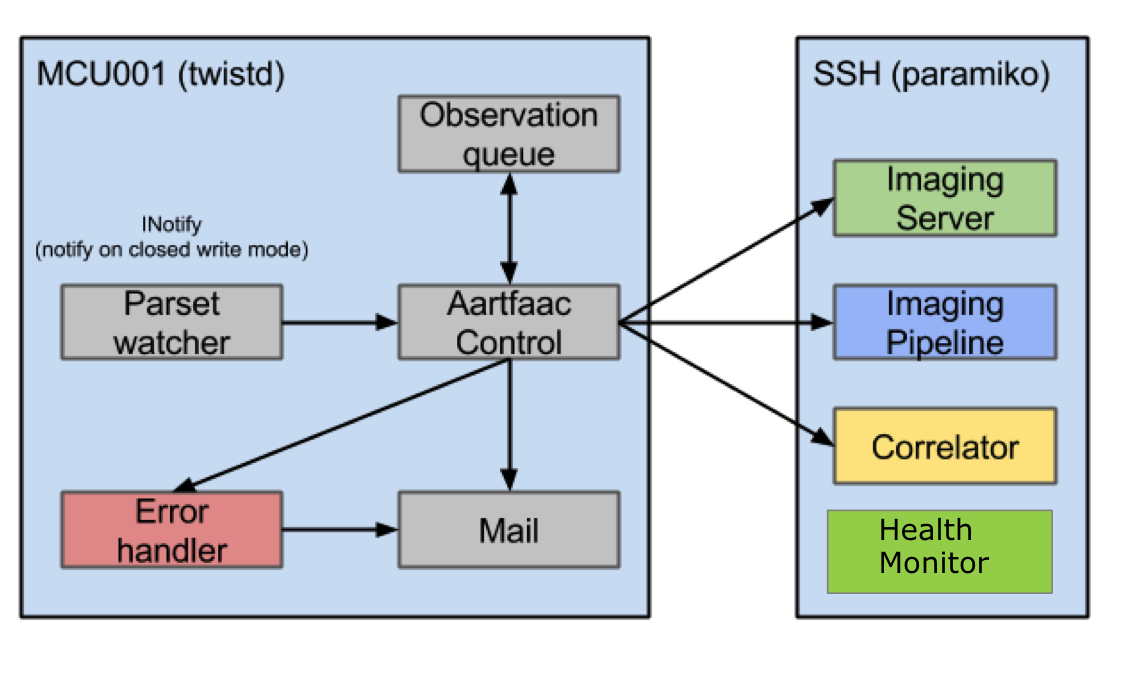
\includegraphics[width=0.25\textwidth]{Figs/control_sys.png}
\caption{The  control  system  architecture  which  interfaces  with  the  LOFAR
  observation scheduling system and triggers AARTFAAC observations.}
\label{fig:afaac_ctrl_sys}
\end{figure*}
Figure  \ref{fig:afaac_ctrl_sys} shows  the  functional blocks  of the  AARTFAAC
control system, and their interface to the LOFAR scheduling system.
\begin {itemize}
 \item {Control system description}
 \item {Interface with LOFAR}
 \item {Monitoring interface: AARTFAAC webpage}
\end {itemize}

\section {\label{sec:results} Commissioning results}
\begin {itemize}
 \item {Overall latency of the system}
 \item {Long term performance of the entire system based on logs.}
 \item {Performance  in various  bit-modes, with  different number  of subbands,
   expected sensitivity.}
 \item {Imaging quality Vs. latency: 6 station to 12 station.}
\end {itemize}

\section {\label{sec:discussion} Discussion}
\subsection {AARTFAAC Scalability}
The AARTFAAC All-Sky  monitor implementation can be scaled up  along the spatial
(number  of dipoles)  or spectral  (processed subbands)  dimensions. A  spectral
scaling will  ultimately be limited  by the ring  network bandwidth to  about 64
subbands (~12  MHz) of 8-bits,  doubling the  current bandwidth. A  spare 10Gbps
link on the uniboards can bring the  extra 32 subbands to the center, where they
can be  processed by an  exact duplicate of  the current correlator  system. The
choice of  a hierarchical  data transpose  results in  the most  efficient final
layout  for  correlation.  In  the  generic case,  following  the  same  design,
additional subbands could be accomodated by increasing the levels in the network
hierarchy  to accomodate  the transpose.  The  final correlation  would then  be
possible for the additional subbands by replication of the frequency multiplexed
hybrid correlator.\\

Keeping the  current bandwidth while increasing  the number of input  dipoles is
also  feasible. The  infiniband  interface  allows another  two  stations to  be
added.  The compute  requirements  would be  almost 30\%  higher,  due to  their
quadratic growth  with number of  input streams.  The correlation  operation has
been tested on the current GPUs for scalability of the input streams, and should
be  able to  cope  with  the requirements  of  the  extra inputs.  Accommodating
stations in addition to  the two mentioned here would likely  require data to be
transferred  between  multiple  CPUs  over  the  GigE  network,  which  will  be
prohibitively slow.

\subsection {\label{subsec:impact_lofar} Impact of sharing dipoles with LOFAR on AARTFAAC}
LOFAR operates using either  the LBA or the HBA antenna at  a time. Further, due
to limited station level electronics for stations within the core, only a subset
of the available station dipoles can be utilized. This implies that the AARTFAAC
telescope  is  dependent  on  LOFAR  for  the  choice  of  antenna  and  station
configuration,  reducing the  availability  for all-sky  monitoring. Within  the
station, only the LBA\_OUTER station configuration is currently deemded suitable
for  real-time imaging.   This mode  of  LOFAR operation  favorable to  AARTFAAC
depends on  the observing  schedule and the  proposed observations.   Table TODO
shows some  statistics from previous cycles  on the fraction of  observing modes
favorable to AARTFAAC. Based on this, it  may be resonable to expect AARTFAAC to
operate TODO fraction of time, typically.

\subsection {Hierarchical swizzling of incoming data:} The voltages are available as
a sampled timeseries  per polarization, with time samples  laid out contiguously
in memory.  For  efficient computing, these need to be  transposed such that the
same  timeslice from  all dipoles  lie  contiguously in  memory. This  operation
involves transposing a matrix  of data with a size NxN, with  N being the number
of data sources.  This memory becomes  inflated by a factor corresponding to the
number  of  timesamples in  the  integration  unit, as  well  as  the number  of
polarizations being  processed. Since the  memory footprint can be  quite large,
this is quite an inefficient operation due to memory read latencies etc.\\

We achieve this by spreading the transpose (or swizzle) operation over the nodes
on our network. This is done in the following manner:
   
The  URI  boards  described  in  Sec.    [TODO]  carry  out  a  first  level  of
transposition by physically  routing a subbands from  a group of 4  dipoles to a
single output. The second stage swizzle is  carried out by the Uniboard. This is
at  the  station level,  and  routes  all dipole  data  from  one station  as  a
contiguously laid out group. Finally, the inter-station swizzling is carried out
by the  CPU host component  of the  correlator. Here, the  PC memory is  used to
rearrange the incoming data and to carry out the transform. The resulting output
is then optimally laid out for correlation over all dipoles of the AARTFAAC, for
every polarization, and over the chosen integration time range.

%\subsection {Dynamic range and precision of computing}
%The 12-bit sampling (TODO: Confirm) provides  for a dynamic range of TODO. These
%raw data samples  are fed into the  hardware first stage PFB,  which carries out
%internal computation  on TODO bit  integer data,  and generates 16-bit  or 8-bit
%complex components (TODO: Is there any normalization at this stage? Why else are
%the actual numbers  so high?). Due to each dipole  sampled output being directly
%operated on without  any beamforming, the 8-bit dynamic range  has been found to
%be adequate for the AARTFAAC application.  Once the data reaches the correlator,
%all computations are carried out with single precision floating points.

\section {\label{sec:conclusion} Conclusions}

\section* {acknowledgements}

This work  was funded  by the ERC  grant <num> awarded  to Prof.   Ralph Wijers,
Universitiet  Van Amsterdam.   We  thank The  Netherlands  Foundation for  Radio
Astronomy  (ASTRON)  for support  provided  in  carrying out  the  commissioning
observations.

\section*{References}

\bibliographystyle{aa}
\bibliography{ref}

\end{document} 
